\subsection{Mechanical Design}
Our sensor node design will require a physical enclosure to protect the sensitive electronic components from damage from various harsh outdoor conditions. To accomplish this we plan on designing a simple 3D printed enclosure out of a plastic material. The material we choose will need to be resistant to constant levels of sun exposure as well as water resistance.

The material we are leaning towards is known as poly ethylene-glycol (PETG). The reason we are looking at using this material for our enclosure is due to the fact that the material is naturally UV resistant. This means it will not degrade over time and become brittle when exposed to direct sunlight over long periods of time. This is critical since our design is intended to be used outdoors, especially in Florida where sunlight is common and intense. PETG also has a high tensile strength that is comparable to ABS, another common 3D printing material. Another benefit of PETG is that it is recyclable and biodegradable, helping to reduce the impact of our design on the environment.

In terms of the design itself, we are planning on creating a simple box with a lid that can be snapped on and off. The design will also need to include holes for the various sensors to be able to complete readings. The design will also need to take into account how the device will be mounted. We intend to make the device light enough that it could be mounted using an off-the-shelf adhesive strip designed for outdoor use. However, we also plan to support other mounting methods, such as including slots on the back of the enclosure where a Velcro strap could be fed through to allow the device to be strapped to a pole or other pole-like structure. Figure \ref{fig:Aether Model} shows the potential design of the Aether node. 

\begin{figure}
    \centering
    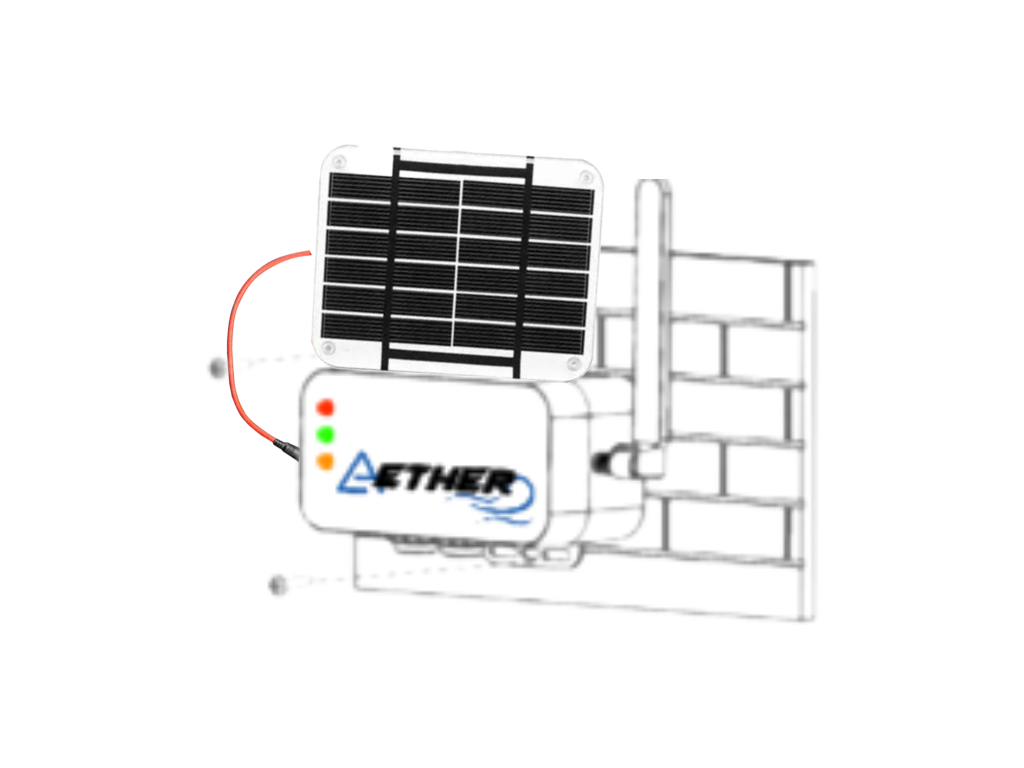
\includegraphics[width=5.5in]{figures/Protoype Design.png}
    \caption{Aether Node Model}
    \label{fig:Aether Model} 
\end{figure}